% -*- TeX-master: "ijcai18.tex" -*-

\section{Motivating example}\label{sec:example}

We provide some background on Kappa and introduce a toy
example motivating the need for counterfactual reasoning in analyzing
the causal structure of simulation traces.

\subsection{Some Background on Kappa}\label{sec:background}

Proteins are complex molecular machines that reversibly tag one
another with molecular flags and reversibly bind each other to form
transient associations.  In this way, proteins come to have ``state"
that can control the interactions they engage in. In Kappa, a protein
is modeled as an abstract \emph{agent} with a name that designates its
\emph{type} and a signature of distinguishable \emph{sites} at which
it can be tagged or bound by other agents. A site can bind at most one
agent at a time and must be in a definite state.
% , each type of agent being described in the model's
% \emph{signature}.

In our illustrative example, we consider two types of agents for which
we use biological nomenclature. One type, $S$, is a substrate that
receives a tag known as a phosphate group in a phosphorylation
interaction. The other, $K$, is a kinase that phosphorylates
$S$. Agents of both types feature a binding site at which they can
bind one another and a site that can be in one of two possible states:
\emph{unphosphorylated} or \emph{phosphorylated}. Thus, agents of type
$K$ also have a phosphorylation state, but for the sake of simplicity
we will have them acquire it ``spontaneously".

A \emph{mixture} is a multiset of agents whose state at each site is
fully specified. A mixture represents the state of a system and can be
thought of as a (potentially large) graph consisting of many connected
components. In a mixture, agents of the same type are distinguished by
a unique global identifier. %(Figure~\ref{fig:mixture}).

\begin{figure}[!h]
  \vskip -0.25cm
  \begin{center}
    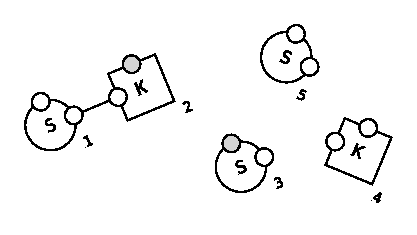
\includegraphics[scale=0.9]{figures/mixture.pdf}
  \end{center}
  \vskip -0.5cm
  \caption{An example of a reaction mixture. Instead of naming sites,
    we here identify them by their position on agents (phosphorylation
    sites are always shown on top). The relative position of agents in
    the figure is insignificant.  Phosphorylated sites are shown in
    gray.  Number labels correspond to global agent identifiers. }
  \label{fig:mixture}
\end{figure}


Interactions between agents are modeled by local rewriting
\emph{rules}.  A rule $r$ is defined by a triple
$(\RLHS{r}, \RRHS{r}, \lambda_r)$, where $\RLHS{r}$ is the left-hand
side specifying a pattern (the pre-condition), $\RRHS{r}$ the
right-hand side (or post-condition), and $\lambda_r$ a firing rate.
The basic idea is that the ``location" at which the mixture matches
$\RLHS{r}$ is rewritten in place by $\RRHS{r}$, changing the state of
the system. (Technically, a rule also requires a function from agents
in $\RLHS{r}$ to agents in $\RRHS{r}$ to make the rewrite
unambiguous.)

% -*- TeX-master: "ijcai18.tex" -*-

\begin{figure}[h]
  \vskip -0.2cm
  \begin{center}
    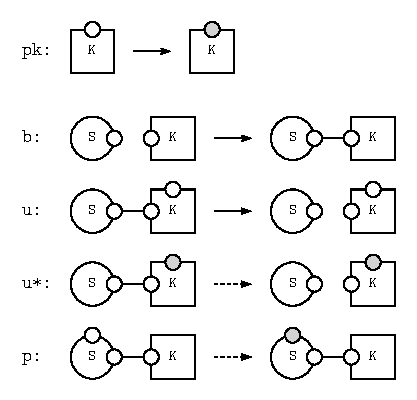
\includegraphics[scale=0.9]{figures/model.pdf}
  \end{center}
  \vskip -0.2cm
  % \caption{A motivating toy model. As usual in Kappa, sites not
  %   mentioned in a rule are left unchanged by it. Instead of naming
  %   sites, we here identify them by their position on an
  %   agent. Phosphorylated sites are shown in gray. Firing rates are
  %   not specified here but dotted arrows indicate \textit{slow}
  %   reactions, whereas solid arrows indicate \textit{fast} reactions.}
  \caption{A motivating toy model. Sites not mentioned in a rule are
    left unchanged by it. \longversion{As in
      Figure~\protect\ref{fig:mixture}, sites are identified by their
      position on an agent.}  Firing rates are not specified, but
    dotted (solid) arrows indicate \textit{slow} (\textit{fast})
    reactions
    $(\lambda_u \gg \lambda_{u^*} \approx \lambda_p)$.}
  \label{fig:model}
\end{figure}


In our toy model, agents are subject to the rules depicted in
Figure~\ref{fig:model}. Rule $b$ states that kinases and substrates
can bind, provided their requisite binding sites are free
(unbound). Note that $\RLHS{b}$ is a pattern: It omits mentioning the
sites that carry phosphorylation state, which are therefore not
considered when matching the mixture to $\RLHS{b}$. Rules $u$ and
$u^{*}$ define unbinding events that depend on the phosphorylation
state of the kinase $K$. The distinction is motivated by kinetics:
Rule $u$ fires at a much faster rate than $u^{*}$. Rule $p$ specifies
that a substrate can be phosphorylated when it is bound to a
kinase. For the sake of simplicity, we model the phosphorylation of a
kinase as a spontaneous process (rule $pk$).

By virtue of the $\lambda_r$, the rules of a model, together with an
initial mixture, constitute a dynamical system that we describe
shortly. We do so in a slightly nonstandard way by introducing the
auxiliary concept of an \emph{event template}. This is to prepare for
the insight in section~\ref{subsec:semantics-refinement} that the
stochastic and deterministic aspects of a model's dynamics can be
cleanly separated, thus enabling counterfactual analysis.

An event template is a pair $(r, \xi)$ where $r$ is a rule and $\xi$ a
function from agents in $\RLHS{r}$ to global identifiers. We say that
$(r, \xi)$ is \emph{realizable} in mixture $m$ if the global
identifiers assigned by $\xi$ exist in $m$ and the agents bearing them
match $\RLHS{r}$. In this case, we write $\TRIGGERABLE{m}{(r, \xi)}$
%(read ``$m$ admits $(r, \xi)$")
and call $\xi$ an \emph{embedding} of
$\RLHS{r}$ into $m$:
\tryinline{\EMBS{r}{m} \eqdef \{ \xi \,:\,
  \TRIGGERABLE{m}{(r, \xi)}\}.}  Whenever $m \vdash (r, \xi)$, we
write $\UPDATE{m}{(r, \xi)}$ the mixture obtained by
realizing $(r, \xi)$, i.e.\@ by rewriting the agents with identifiers
in the codomain of $\xi$ into $\RRHS{r}$. The realization of an event
template at a particular time creates an (actual) \emph{event},
formally defined as a pair $(e, t)$ with $e$ an event template and $t$
its time of realization.

A model induces a continuous-time Markov chain (CTMC) over the
set of reachable mixtures, where state $m$ transitions to state
$\UPDATE{m}{(r, \xi)}$ at rate $\lambda_r$ for every event template
$(r, \xi)$ that is realizable in $m$. The rate of leaving state $m$ by
an application of rule $r$ is called the \emph{activity} $\alpha_r(m)$
of rule $r$ in
% \ifshort $m$: \else
mixture $m$ and is equal to the product of the rule's firing rate by
the number of embeddings of $\RLHS{r}$ into $m$:
% \fi
$\alpha_r(m)=\lambda_r|\EMBS{r}{m}|$. For example, in
Figure~\ref{fig:mixture}, rule $b$ has activity $2\lambda_b$ and rule
$u$ has activity $0$. The \emph{total activity} of a mixture is defined
as $\alpha(m)=\sum_r\alpha_r(m)=\sum_r\lambda_r|\EMBS{r}{m}|$.
% In terms of CTMC, it corresponds to the total transition rate of $m$.

The CTMC induced by a model can be simulated
with the \emph{Doob-Gillespie algorithm} \cite{gillespie1977exact},
which loops over the following steps:
\begin{inparaenum}[(1)]
\item draw a time interval $\delta$ to the next event from an
  exponential distribution with parameter $\alpha(m)$ and increment
  the simulated system time by $\delta$,
\item draw a rule $r$ with probability $\alpha_r(m)/\alpha(m)$ and
\item pick uniformly an embedding $\xi \in \EMBS{r}{m}$ of $L_r$ into
  $m$ and realize the event template $(r, \xi)$.
\end{inparaenum}
This algorithm is efficiently implemented for rule-based models in
Kappa as described in
\cite{DanosEtAl-APLAS07,BoutillierEK17}\longversion{; it is available
  at kappalanguage.org}. It outputs a sequence of events,
called a \emph{trace}.


\longversion{\begin{algorithm}
\caption{Doob-Gillespie algorithm}\label{alg:gillespie}
\begin{spacing}{1.2}
\begin{algorithmic}
\vspace{0.2cm}
  \STATE $t \gets 0$
  \STATE $m \gets\ $ initial mixture
  \vspace{0.1cm}
  \WHILE{ $t < t_\text{\,end}$ }
      \vspace{0.1cm}
      \STATE $\alpha \gets \sum_r {\lambda_r |\EMBS{r}{m}|}$
      \vspace{0.1cm}
      \STATE draw $\delta \sim \textsc{Exp}(\alpha) $
      \STATE $t \gets t + \delta$
      \STATE draw a rule $r$ with probability
      $\propto \ \lambda_r |\EMBS{r}{m}|$
      \STATE draw an embedding $\xi$ uniformly in $\EMBS{r}{m}$
      %\STATE update $m$ by triggering event $((r, \xi), t)$
      \STATE $m \gets \UPDATE{m}{(r, \xi)}$
      \STATE log event $((r, \xi), t)$
  \ENDWHILE
\vspace{0.1cm}
\end{algorithmic}
\end{spacing}
\end{algorithm}}

\subsection{Where Existing Analysis Falls Short}
\label{subsec:dumb-story}

% What about asking the question for the specific trace to make it
% clearer we are talking about actual causality ?

Consider our toy model and assume, for the sake of illustration, an
initial mixture $I$ with only a single kinase and a single substrate
whose sites are unbound and unphosphorylated. We then ask: Starting
from $I$, \emph{how} is $p$ typically achieved? We are not merely
looking for an account of reachability but for a causal explanation,
i.e.\@ a collection of events connected by causal influences.

For example, a simulation might produce the following trace (events
are labelled by the rules that induced them):
\begin{align}
  \label{example-trace} 
  b,\ \ u,\ \ pk,\ \ b,\ \ p,\ \ u^{*},\ \ \cdots
\end{align} 
Current techniques
\cite{DBLP:conf/fsttcs/DanosFFHH12,DanosEtAl-CONCUR07} generate a
causal account by first computing a \emph{sub-trace} of
(\ref{example-trace}) that is
\begin{inparaenum}[(i)]
\item \emph{valid} in the sense that each of its events can be
  triggered in turn starting from the initial mixture and
\item \emph{minimal} in the sense that none of its valid sub-traces
  features $p$.
\end{inparaenum}
The relations of enablement among events in the minimal sub-trace
yield a directed acyclic graph. Although trivial in our toy example,
minimization is an NP-hard problem. Carrying out this approach on
(\ref{example-trace}), one notes that the first occurence of $b$ sets
the necessary conditions for $p$, but these are subsequently undone by
$u$ only for the second occurrence of $b$ to re-introduce them. This
illustrates why minimization compresses a trace into events that are
\emph{necessary} for the outcome---which requires eliminating futile
cycles. In our case, the causal account for $p$ starts with the
initial condition, symbolized by the \emph{init} event, and skips to
the last $b$ before the $u$. Figure~\ref{fig:dumb-story} depicts the
resulting explanation graph, whose arrows denote enablement as defined
informally in section~\ref{sec:intro} and formally in
section~\ref{sec:inhibition}.

\begin{figure}[H]
  \vskip -0.8cm
  \begin{center}
    \includegraphics[scale=0.7]{figures/dot/dumb-story.pdf}
  \end{center}
  \vskip -1cm
  \caption{A causal explanation for $p$ in trace
    (\ref{example-trace}).  Events are labelled by the rules that
    induced them. The \emph{init} node corresponds to a special event
    that sets the mixture to its initial state.  }
  \label{fig:dumb-story}
\end{figure}


The problem is that the explanation depicted in
Figure~\ref{fig:dumb-story} fails to recognize the critical role of
$pk$ in the original trace. Given the rules of the model, one notes
that $p$ is slow and the average time that $K$ remains bound to $S$
depends on the phosphorylation state of $K$. The kinase $K$ is
phosphorylated in event $pk$, causing the complex between $K$ and $S$
to be sticky, giving the slow phosphorylation $p$ a chance to
occur. It seems reasonable to assert that $p$ would probably not have
happened had $pk$ not happened, since the opportunity for $p$ would
have been curtailed by a fast unbinding event. Thus, $pk$ should be
part of the explanation, although it neither enables $b$ nor $p$
directly (both rules are independent of $K$'s phosphorylation
state). Reasoning of this kind is \emph{counterfactual}
\cite{lewis1974causation,pearl2009causality}.

In section~\ref{sec:counterfactual}, we give a rigorous semantics to
this line of reasoning and introduce an algorithm for simulating
counterfactual scenarios. In section~\ref{sec:inhibition}, we show how
counterfactual dependencies between events can be systematically
explained in terms of a combination of enablement and prevention
arrows, leading to the explanation shown in Figure~\ref{fig:cex}. 
%for the counterfactual dependency between $p$ and $pk$ in our example.
